\documentclass[11pt,a4paper]{article}
\usepackage[utf8x]{inputenc}
\usepackage{ucs}
\usepackage{amsmath}
\usepackage{mathtools}
\usepackage{amsfonts}
\usepackage{amssymb}
\usepackage{tabu}
\usepackage{graphicx,xspace}
\usepackage{float}
\usepackage{url}

\usepackage{color}
\usepackage{xcolor}
\usepackage{listings}

\usepackage[margin=1in]{geometry}

\usepackage{titling}
\setlength{\droptitle}{-1in}


\usepackage[margin=1in]{caption}
\usepackage{courier}

\setlength{\parindent}{0.2in}

\title{The Domain Name System (DNS) \vspace{-2ex}}
\author{originally created by Jo\v{z}i McKiernan}
\date{}

\begin{document}

\maketitle



\section{Introduction}

\indent\indent In this lab you will learn about the Domain Name System, or DNS.
The DNS is a hierarchical system for giving names to computers on the Internet and for matching computers' names to their numerical IP addresses. 
%The IP address space exists alongside the domain name hierarchy in the DNS, and the IP addresses are used to locate the hosts on the network.
The DNS is implemented by a communication protocol and a hierarchical system of DNS servers.

% DNS servers are servers that store the DNS records for a particular domain name.

\subsection{Organization}
\indent\indent Under the DNS, the Internet is organized into a hierarchy of domains. 
Each computer, or \textit{host} has its own domain name that includes the names of all of its parent domains.
A complete domain name consists of a series of labels separated by dots. 
The domain labels are listed in hierarchical order from right to left.
That is, the highest-level domain is listed the farthest right. 
For example:

\begin{center}
$\underbrace{www.}_{\text{lowest-level domain}}google.\underbrace{com}_{\text{highest-level domain}}$



\end{center}
In this case, $com$ is the top-level domain (TLD), $google$ is the middle-level domain, and $www$ is the lowest-level domain. 
Notice the dots between each label in the domain name.
The domain name hierarchy can be visualized somewhat like Figure \ref{fig:hierarchy}.

\begin{figure}[H]
	
    \centering
    	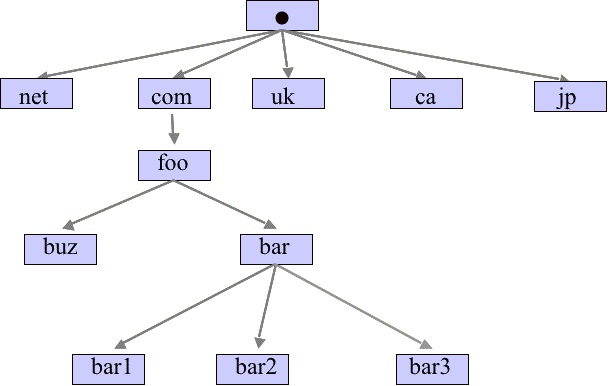
\includegraphics[width=0.5\textwidth]{dns.jpg}
    \caption{Hypothetical domain name hierarchy. At the top of the tree is the root domain ``." The top-level domains are immediately below the root domain on the tree. Below the top-level domains you can see a number of subdomains.}
    \label{fig:hierarchy}
\end{figure}

The DNS stores information about each domain in \textit{resource records (RRs)}. 
Each type of RR stores a different piece of information about a domain name, such as its IP address or the mail transfer agent used by the domain. 
The DNS relies on DNS name servers to store these RRs.
Each DNS name server is given a zone of authority in the domain name space for which it is responsible. 
The server contains all the RRs for all of the domain names within its zone of authority. 
An example of zones of authority within the domain name hierarchy can be seen in Figure \ref{fig:zone}.

\begin{figure}[H]
	
    \centering
    	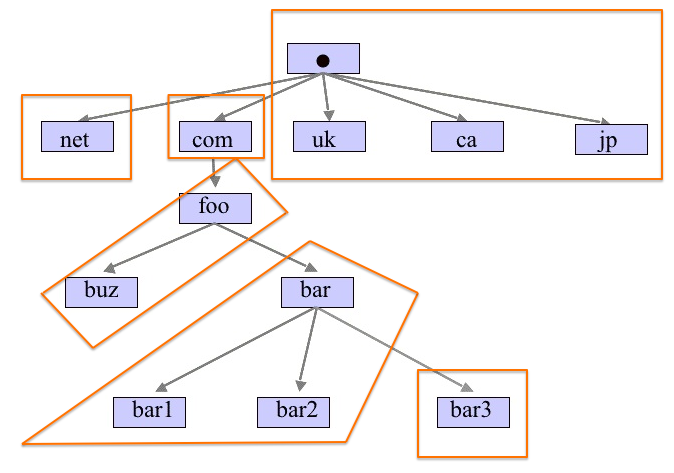
\includegraphics[width=0.6\textwidth]{KkU6GWrzYGTS7GpSURtX7Dh9tFX_BjWGijM_HnewKXw.png}
    \caption{Hypothetical zones of authority. Each box represents a zone of authority administered by a distinct name server. The name server is responsible for the RRs for every domain name within its zone. }
    \label{fig:zone}
\end{figure}

To improve reliability, at least two servers are assigned to maintain the
records for each domain name.  Always, one of the name servers dedicated to a
zone will be an authoritative name server, a server that updates its RRs from
authoritative sources only. (See Section 2 for more information about RRs).

The computers that run DNS have their own IP addresses, too, and their own 
resource records. In
addition to RRs for itself and for all of the names within its zone, a
DNS name server stores records pointing to the authoritative name
servers that manage child zones. For instance, in Figure~\ref{fig:zone}, the
name server managing the zone with foo and buz also contains a record
pointing to the name server that manages the zone containing bar. The
name server managing the zone with . also contains records pointing to
the name servers managing com and net. In real life, there are thirteen
root name servers worldwide that manage the Internet~\cite{DNS}
This number might seem small, given that these servers are the root name
servers for the whole of the Internet. However, the number seems more
reasonable when you consider that the root name servers have fairly
small amounts of RRs since they have delegated the lower parts of the
zone of authority to other name servers. You can see this sort of
delegation in Figure~\ref{fig:zone}. While the root name server in 
Figure~\ref{fig:zone} contains RRs for itself, ., uk, jp, and ca as well as
pointers to the servers for com and net, it does not contain pointers or
other records for foo and bar. The root nameserver has delegated part of
its zone of authority to the com name server and the net name server,
and the com name server has in turn delegated some of its zone of
authority to the foo name server.

\subsection{Query Process}
\indent\indent In order to access the records contained in the DNS, a user or a device must pose a query.
Once the query is posed, the local system (i.e., the user's computer and software) tries to answer the query first. 
If this attempt is unsuccessful, the query gets passed to a resolver that attempts to resolve the query by systematically checking name servers for the correct RR. 
If no applicable RR is found, an error is returned. 

\begin{figure}
	
    \centering
    	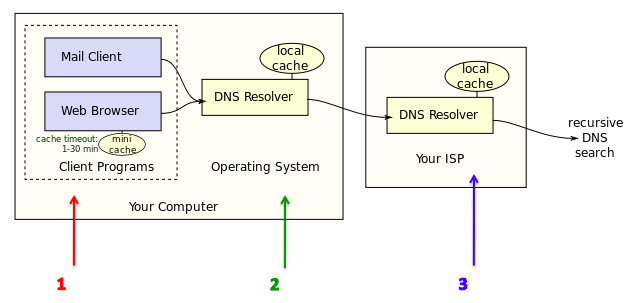
\includegraphics[width=0.75\textwidth]{query2.png}
    \caption{The first part of the query-resolving process. The large box on the left represents the computer and the programs running inside of it. In step 1, the client application tries to resolve the query from the records stored in its cache. In step 2, the local resolver within the computer tries to resolve the query from its cache. The operating system translates the query from the user's request (such as entering ``www.google.com" in a search bar) to a DNS message format. Finally, if both steps 1 and 2 fail to resolve the query, the query is passed on to a recursive resolver that will perform a recursive search of name servers until it can resolve its query. The recursive resolver is usually provided by an Internet Service Provider (ISP). }
    \label{fig:local}
\end{figure}

For example, perhaps a user enters a query by opening a browser window and searching for a website by domain name. 
This kind of query is equivalent to looking up an IP address from a domain name.
First, the client application will try to resolve the query by checking for the record and address in their cache (Step 1, above, in Figure \ref{fig:local}).
If that fails, the operating system will translate the application's query into a DNS message and give it to the local resolver (still within the computer).
The local resolver will then try to resolve the query from its cache of records (Step 2 in Figure \ref{fig:local}).
If the address is not found, the local resolver sends the query to a recursive resolver, generally maintained by an Internet Service Provider. 
The recursive resolver checks its own cache and records for the response to the query (Step 3 in Figure \ref{fig:local}). 
If it doesn't find the answer, it queries other name servers recursively until it resolves the query, starting with the root name server. 
The recursive search process is shown in Figure \ref{fig:remote}.

\begin{figure}
	
    \centering
    	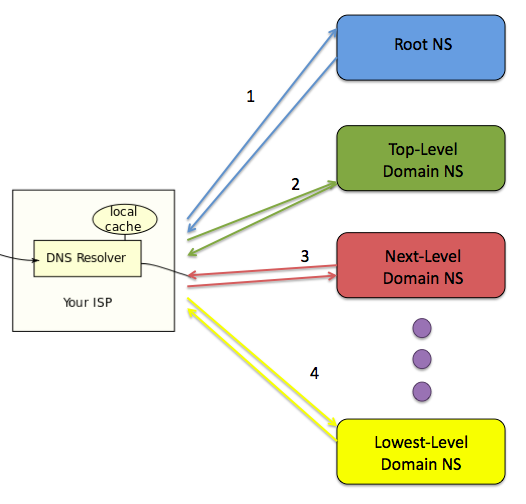
\includegraphics[width=0.5\textwidth]{query3.png}
    \caption{The second part of the query-resolving process. The box on the left represents the recursive resolver. In step 1, the recursive resolver tries to resolve the query from the records contained in root (blue box). If root cannot answer the query, it provides the IP address of the next-level name server (green box). In step 2, the resolver goes to the provided IP address of the green name server and poses the query again. If the green name server cannot answer the query, it returns the IP address of the next-level name server (red box). In step 3, the resolver goes to the provided IP address for the red name server and poses the query again. If the red name server cannot answer the query, it provides an IP address for the next level name server. Step 3 repeats until a record is found or the bottom of the tree is reached. In either case, the resolver goes to the lowest-level-necessary name server (step 4). This name server returns either the record or an error to the recursive resolver. The recursive resolver then passes this answer back to the computer.}
    \label{fig:remote}
\end{figure}

As you can see, the recursive resolver begins by querying the root name server.
If the root does not have the correct record, it returns the IP address of the correct top-level domain name server for the query (Step 1 in Figure \ref{fig:remote}).
Then the recursive resolver goes to the returned IP address and repeats the query.
If the top-level domain name server does not have the correct record, it returns the IP address of the next-level domain name server (Step 2 above).
The recursive resolver then travels to the newly provided IP address and tries to resolve the query again.
If the name server does not have the correct record, it returns the IP address of the next-level domain name server (Step 3 above).
Step 3 repeats indefinitely until the record is found.
In step 4, when the recursive resolver poses the query to the lowest-level domain name server, the correct record is found and returned to the recursive resolver.
The recursive resolver returns the answer to the local resolver in the computer, and the local resolver returns the record to the client application by way of the operating system.

Most queries seek a ``standard" lookup of a record from a domain name. 
However, the DNS also handles reverse lookups to find a domain name from an IP address.
In this case, the DNS client (i.e., an app) converts the IP address into special notation depending on whether it is an IPv4 or an IPv6 address. 
Then the resolver searches for a pointer (PTR) record for the IP address starting at root and the top-level IP address name server, either in-addr.arpa (IPv4)or ip6.arpa (IPv6).
The top-level name server then returns the address of the name server for the next-lowest domain, and so on and so forth until the name server authoritative for the lowest-level domain is reached.
Then the name server finds a PTR record for the original IP address and returns the correct domain name.

Address queries are the most common queries that the DNS handles, but it also has several other functionalities due to the detailed resource records it maintains.
Some of these are discussed in more detail below. 


\section{RESOURCE RECORDS}
\indent\indent The DNS keeps a variety of resource records (RRs) for each domain name. 
A full record consists of six types of information: name, type, class, TTL, rdlength, and rdata. 
Name is the domain name of the subject of the record, i.e. knuth's resource records have ``knuth.cs.hmc.edu" in their name field. 
Type is the type of record, described in more detail below.
Each record also has a class in addition to a type.  
Internet (IN) is the class used for normal computers and devices connecting to the Internet, but there are other classes including Chaos (CH) and Hesiod (HS).
(Chaos is a class referring to another, older domain system, and Hesiod is a class that provides DNS-like access to some databases.)
TTL is the time before the record expires. (More on that in a minute.)
Rdlength is the length of the rdata section, and rdata is the record itself.

The TTL serves an important role in helping to keep the DNS up-to-date.
Since resolvers and computers use caching to store RRs that have been recently accessed, the overall speed of DNS lookups is greatly improved. 
However, problems arise when a RR changes because the cache is not automatically updated. 
Sometimes, an incorrect RR will be returned from a cache. 
To help control this, every DNS response is stored for an amount of time called time to live, abbreviated TTL. 
The TTL can be set by the sysadmin, and the DNS framework supports TTLs from 0 seconds to about 68 years~\cite{DNS}. 
When an RR reaches its TTL, it expires and is discarded. 
Until that happens, however, the record remains in a cache and is consulted when a corresponding query is received. 
It is important to remember that the DNS is not updated universally when changes occur.

There are more than fifty possible RR types. 
Each contains different information about a domain name, and each is looked up in the same manner.
Some of the most important ones are summarized in the table below.
For a more complete list, see\\ 
\url{http://en.wikipedia.org/wiki/List_of_DNS_record_types}.

\begin{center}
\begin{tabular}{|l|l|p{7cm}|}
\hline
\textbf{Type} & \textbf{Description} & \textbf{Details} \\ \hline
A & Address record & Returns a 32-bit IPv4 address, most commonly used to map hostnames to an IP address of the host, but also used for other things.\\ \hline
AAAA & IPv6 address record & Returns a 128-bit IPv6 address, most commonly used to map hostnames to an IP address of the host.\\ \hline
CNAME & Canonical name record & Alias of one name to another: the DNS lookup will continue by retrying the lookup with the new name. \\ \hline
DNAME & Delegation Name & DNAME creates an alias for a name and all its subnames, unlike CNAME, which aliases only the exact name in its label. Like the CNAME record, the DNS lookup will continue by retrying the lookup with the new name. \\ \hline
LOC & Location record & Specifies a geographical location associated with a domain name. \\ \hline
MX & Mail exchange record & Maps a domain name to a list of message transfer agents for that domain.\\ \hline
NS & Name server record & Delegates a DNS zone to use the given authoritative name servers.\\ \hline
PTR & Pointer record & Pointer to a canonical name. Unlike a CNAME, DNS processing does NOT proceed, just the name is returned. The most common use is for implementing reverse DNS lookups, but other uses include such things as DNS-SD.\\ \hline
RP & Responsible person & Information about the responsible person(s) for the domain. Usually an email address with the @ replaced by a ``."\\ \hline
SOA & Start of [a zone of] authority record & Specifies authoritative information about a DNS zone, including the primary name server, the email of the domain administrator, the domain serial number, and several timers relating to refreshing the zone.\\ \hline
TXT & Text record & Originally for arbitrary human-readable text in a DNS record. Since the early 1990s, however, this record more often carries machine-readable data, such as specified by RFC 1464, opportunistic encryption, Sender Policy Framework, DKIM, DMARC, DNS-SD, etc.\\ 
\hline
\end{tabular}
\end{center} 



\section{DNS MESSAGES}
\indent \indent There are two types of DNS messages: queries and replies.
Both have the same format with five sections: header, question, reply, authority, and additional. 

You can see these queries and responses using \verb|dig|, the \underline domain \underline information \underline groper. 
%\verb|dig| is part of the \verb|bind-tools| package. 
\newpage
To pose a query with \verb|dig|, type
\begin{lstlisting}[basicstyle=\ttfamily, backgroundcolor = \color{lightgray}, language = bash, xleftmargin = 0cm, framexleftmargin = 1em]
dig @servername hostname RECORDTYPE
\end{lstlisting}
The server name is optional; the computer will automatically go to the servers listed in /etc/resolv.conf if none is supplied.
The hostname is the domain name of the address you're looking for, e.g., www.google.com, or knuth.cs.hmc.edu.
The record type is the type of record you want to fetch. 
By default it fetches the IPv4 address for the domain name indicated (resource record type A).
You might also search for the IPv6 address, type AAAA.
See the \verb|man| page for \verb|dig| for more details about each argument, and for information about options such as reverse lookup. 

Now try running 
\begin{lstlisting}[basicstyle=\ttfamily, backgroundcolor = \color{lightgray}, language = bash, xleftmargin = 0cm, framexleftmargin = 1em]
dig crispy.sys.cs.hmc.edu | less
\end{lstlisting}

The command should produce an output similar to this:
\begin{lstlisting}[basicstyle=\ttfamily, backgroundcolor = \color{lightgray}, language = bash, xleftmargin = 0cm, framexleftmargin = 1em]
; <<>> DiG 9.6-ESV-R4-P3 <<>> crispy.sys.cs.hmc.edu
;; global options: +cmd
;; Got answer:
;; ->>HEADER<<- opcode: QUERY, status: NOERROR, id: 20877
;; flags: qr rd ra; QUERY: 1, ANSWER: 1, AUTHORITY: 1, ADDITIONAL: 1

;; QUESTION SECTION:
;crispy.sys.cs.hmc.edu.		IN	A

;; ANSWER SECTION:
crispy.sys.cs.hmc.edu.	86400	IN	A	134.173.43.165

;; AUTHORITY SECTION:
sys.cs.hmc.edu.		86400	IN	NS	crispy.sys.cs.hmc.edu
.

;; ADDITIONAL SECTION:
crispy.sys.cs.hmc.edu.	86400	IN	AAAA	2620:102:2001:903:1a0
3:73ff:fe2a:541e

;; Query time: 11 msec
;; SERVER: 134.173.254.23#53(134.173.254.23)
;; WHEN: Mon Jul  7 10:55:33 2014
;; MSG SIZE  rcvd: 97
\end{lstlisting}

First, you will see some information about the command itself, such as the \verb|dig| version and the domain name you included.

The \verb|->>HEADER<<-| section gives information about what the rest of the message contains, such as how many answers or records it fetched, and the id number of the query. 
The id number is used by the name servers to match queries with their responses. 

Next you may see the \verb|OPT| pseudosection. 
You can more or less ignore it; it is just there to provide information for EDNS, an extension of the DNS that allows several parameters to be bigger than normal. 

The \verb|QUESTION SECTION| displays the domain name and record type you're searching for as well as the class of the domain name. 
If you were searching for a record type other than \verb|A|, this would appear here as well as in your original query.

The \verb|ANSWER SECTION| gives the resource records that you queried for.
There can be multiple records if you asked for multiple types of records or if the hostname has multiple IP addresses or other records associated with it. 
The answer has the format 
\begin{lstlisting}[basicstyle=\ttfamily, backgroundcolor = \color{lightgray}, language = bash, xleftmargin = 0cm, framexleftmargin = 1em]
search.term 	TTL 	CLASS 	TYPE	 RDATA
\end{lstlisting}
where \verb|RDATA| is the record (answer) you're looking for.

The \verb|AUTHORITY SECTION| lists the authoritative name servers that were used in resolving the domain name in your query and some other information about the servers.
The records in this section generally have the format
\begin{lstlisting}[basicstyle=\ttfamily, backgroundcolor = \color{lightgray}, language = bash, xleftmargin = 0cm, framexleftmargin = 1em]
domain.name 	TTL 	CLASS 	TYPE (NS)	 auth.server.name
\end{lstlisting}

The \verb|ADDITIONAL SECTION| gives any additional information that was needed in the process of resolving the query, such as the IP addresses of the authoritative name servers used to resolve your query.
Your computer doesn't know how to reach the authoritative name servers unless those IPs are provided to it in the additional section. 
This kind of additional record is called a glue record.
In the example above, you can see an additional record containing the IPv6 address for crispy.

You can set an alias for your computer's domain name in the file /etc/hosts, assuming you have the correct permissions. 
/etc/hosts contains alias-to-IP address mappings for local hosts.
If you navigate to your /etc/hosts file, you should see several aliases for your machine at 127.0.0.1.
There may also be aliases for other computers on the sys.cs.hmc.edu network.
Whether or not these aliases are used for DNS lookup depends on the settings in /etc/host.conf.
Lookups will be resolved according to the order specified by the ``order" keyword in /etc/host.conf. 
If ``hosts'' is not the first thing listed after ``order,'' DNS lookup will occur according to other methods before referring to the /etc/hosts file.

Now try running
\begin{lstlisting}[basicstyle=\ttfamily, backgroundcolor = \color{lightgray}, language = bash, xleftmargin = 0cm, framexleftmargin = 1em]
dig knuth.cs.hmc.edu | less
\end{lstlisting}
and answer the following questions.

\begin{enumerate}
\item What is the IPv4 address of knuth?
\item Which are the authoritative name servers for knuth?
\item What is the IPv6 address of kay?
\item What command would you run to do a reverse lookup for knuth? (Hint: see man page for \verb|dig|)
\end{enumerate}

If you'd like more detailed information about the DNS, you can check out the
resources at the end of this document, and you can read chapter 16 of \textit{
Linux Administration, A Beginner's Guide, Sixth Edition}.

If you're interested in some applications that rely on DNS, you might check out:
\begin{description}
\item[\texttt{ping}] Is a host available?
\item[\texttt{traceroute}] How do I get from one computer to another, over the
Internet?
\end{description}

If you're interested in DNS and security, you might check out ``DNS hijacking''
or ``DNS amplification''.

\textbf{As with all things related to system administration, be responsible with
this information and these tools. It's usually okay to run one instance of ping
against a host or one instance of traceroute. But launching a flood of requests
against another system is never okay. Neither is it okay to compromise the
security or availability of a host, unless you have permission from all parties
responsible for that host.}

\begin{thebibliography}{15}
\addtolength{\leftmargin}{0.2in}
\setlength{\itemindent}{-0.2in}

    \bibitem {DNS} ``Domain Name System." \emph{Wikipedia}.Wikimedia Foundation, Inc. 25 June 2014. Web. 26 June 2014. 
    \bibitem{msg} Heinlein, Paul. ``DiG HOWTO." \emph{madboa.com}. n.p. 11 May 2006. Web. 26 June 2014.
    \bibitem{RR} ``Types of Resource Records." \emph{Wikipedia}.Wikimedia Foundation, Inc. 26 April 2014. Web. 26 June 2014. 
    \bibitem{msoft} ``How DNS Query Works." \emph{TechNet}. Microsoft. 21 January 2005. Web. 26 June 2014.
    \bibitem{queryinfo} ``Chapter 15: DNS Messages." \emph{zytrax.com} ZyTrax, Inc. 10 December 2013. Web. 26 June 2014.
    \bibitem{edns} ``Extension Mechanisms for DNS." \emph{Wikipedia}. Wikimedia Foundation, Inc. 16 June 2014. Web. 26 June 2014. 
   
\end{thebibliography}

\end{document}